% Generated by scripts/paper_figures.py from frozen files. Do not edit by hand.
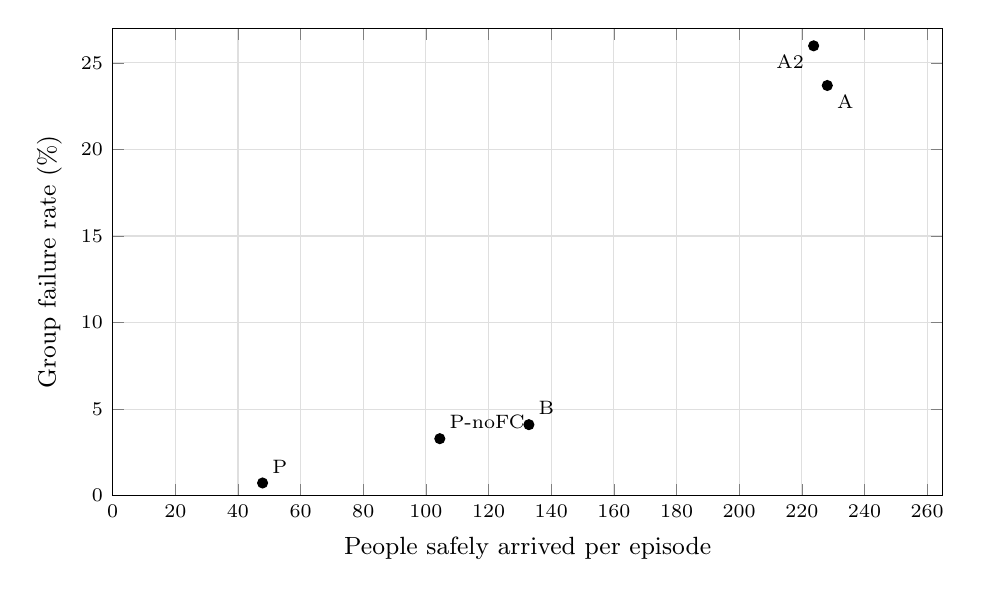
\begin{tikzpicture}
  \begin{axis}[width=\columnwidth, height=0.62\columnwidth,
    xlabel={People safely arrived per episode}, ylabel={Group failure rate (\%)},
    xmin=0, xmax=265, ymin=0, ymax=27, grid=major, grid style={gray!25},
    tick label style={font=\scriptsize}, label style={font=\small}]
    \addplot[only marks, mark=*, mark size=1.8pt] coordinates {
      (228.108,23.692) [A]
      (223.750,25.983) [A2]
      (132.867,4.100) [B]
      (47.858,0.731) [P]
      (104.425,3.290) [P-noFC]
    };
    \node[anchor=north west,font=\scriptsize] at (axis cs:228.108,23.692) {A};
    \node[anchor=north east,font=\scriptsize] at (axis cs:223.750,25.983) {A2};
    \node[anchor=south west,font=\scriptsize] at (axis cs:132.867,4.100) {B};
    \node[anchor=south west,font=\scriptsize] at (axis cs:47.858,0.731) {P};
    \node[anchor=south west,font=\scriptsize] at (axis cs:104.425,3.290) {P-noFC};
  \end{axis}
\end{tikzpicture}
